%!TEX root = slides.tex

\title{Graph Theory}
\subtitle{}
\author{ian.mcloughlin@gmit.ie}
\date{}


\begin{frame}
	\titlepage
\end{frame}

\begin{frame}
	\frametitle{Topics}
	\tableofcontents
\end{frame}

\section{Graphs}

\begin{frame}{Seven Bridges of K{\"o}nigsberg}
	\begin{center}
		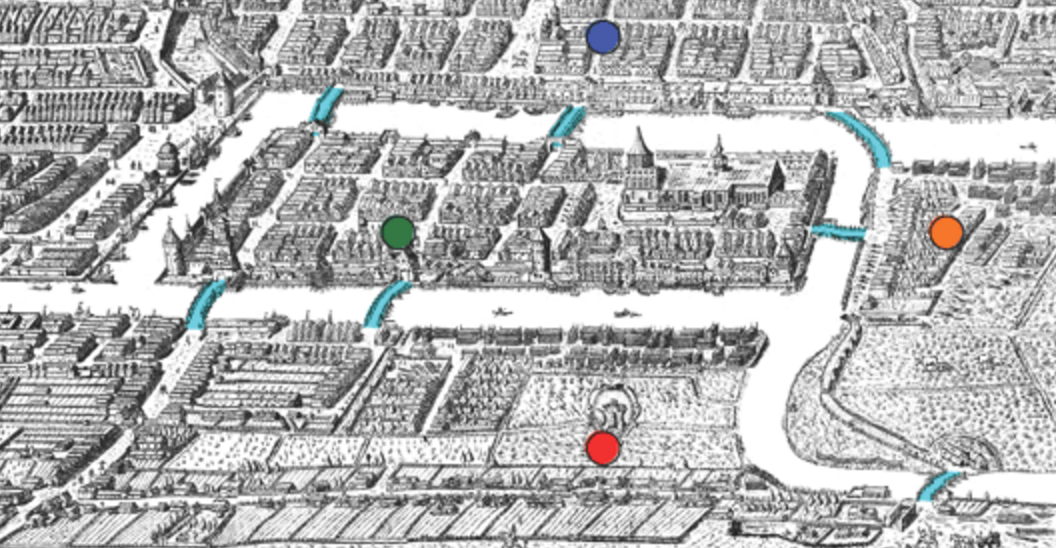
\includegraphics[width=9cm]{img/konigsberg.png}
	\end{center}
	Is it possible to walk through the city crossing each of the seven bridges once and only once?
		\citeurl{www.nature.com/nbt/journal/v29/n11}
\end{frame}

\begin{frame}{Leonhard Euler}
  \begin{columns}
    \begin{column}{0.25\textwidth}
      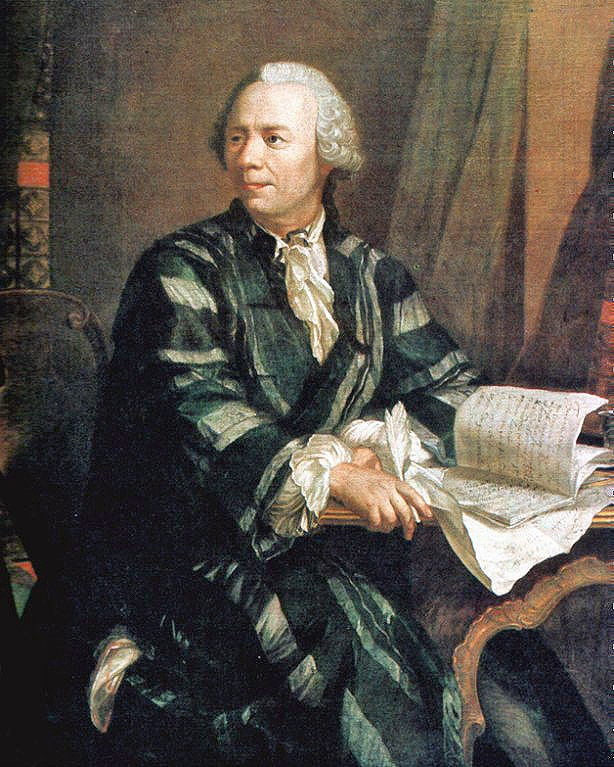
\includegraphics[height=1.8in]{img/euler.jpg}
    \end{column}
    \begin{column}{0.6\textwidth}
      \begin{itemize}
    	 \item Born 1707 in Basel, Switzerland.
        \vspace{0.25cm}
    	 \item Euler's identity: $\mathrm{e}^{i \pi} + 1 = 0$.
        \vspace{0.25cm}
    	 \item Solved the Bridges of K{\"o}nigsberg problem.
        \vspace{0.25cm}
        \item It's not possible to cross all bridges once and once only.
      \end{itemize}
    \end{column}
  \end{columns}
  \citeurl{https://en.wikipedia.org/wiki/Leonhard\_Euler}
\end{frame}

\begin{frame}{Graph of K{\"o}nigsberg}
  \begin{adjustbox}{max width={0.9\textwidth},center} 
    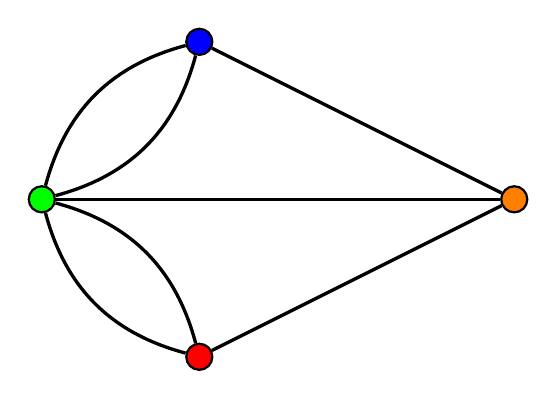
\begin{tikzpicture}
			\begin{scope}[every node/.style={circle,thick,draw}]
		    \node[fill=green] (A) at (0,0) {};
		    \node[fill=blue] (B) at (2,2) {};
		    \node[fill=orange] (C) at (6,0) {};
		    \node[fill=red] (D) at (2,-2) {};
			\end{scope}
			\begin{scope}[every edge/.style={draw=black,very thick}]
		    \path (A) edge[bend right=30] (B);
    		\path (A) edge[bend left=30] (B);
		    \path (A) edge[bend right=30] (D);
		    \path (A) edge[bend left=30]  (D);
		    \path (B) edge (C);
		    \path (A) edge (C);
		    \path (D) edge (C);
	    \end{scope}
    \end{tikzpicture}
  \end{adjustbox}
\end{frame}


\begin{frame}{Graph definition}
	\begin{definition}
	A \emph{graph} consists of a finite set $V$ and a set $E$ of 2-subsets of $V$.
	\end{definition}
	\vspace{0.25cm}
	\begin{description}
		\item[Vertices] -- the elements of the set $V$ are called vertices.
		\vspace{0.25cm}
		\item[Edges] -- the elements of $E$ are called edges.
		\vspace{0.25cm}
		\item[$G = (V,E)$] -- this is the way we write the graph $G$ consists of the vertex set $V$ and the edge set $E$.
	\end{description}
\end{frame}

\begin{frame}{Sets of K{\"o}nigsberg}
$$ V = \{Green, Blue, Orange, Red\} $$
\begin{align*}
E = \{&\\
			&\{Green, Blue\}, \{Green, Blue\}, \{Green, Red\},\\
      &\{Green, Red\}, \{Blue, Orange\}, \{Green, Orange\},\\
      &\{Red, Orange\}\\
      \}&
\end{align*}
\end{frame}

\begin{frame}{Adjanceny list}
	\begin{center}
	\begin{tabular}{l|l|l|l}
	Green & Blue & Orange & Red \\
	\hline
	Blue & Green & Blue & Green \\
	Orange & Orange & Green & Orange \\
	Red & & Red & 
	\end{tabular}
	\end{center}
\end{frame}

\begin{frame}{Defining different types of graphs}
	
	\begin{block}{Our definition of a graph}
	The definition given above for a graph is consistent with looped edges, but not directed edges and not repeated edges. We only need to make small changes to the definition of a graph to allow for directed edges and repeated edges.
	\end{block}
	
	\begin{description}
		\item[Repeated edges] are edges that start and end at the same vertices.
		\item[Directed edges] are edges where a direction is added.
		\item[Looped edges] begin and end at the same vertex.
	\end{description}
	
	The application will determine the definition we want to use.
\end{frame}


\begin{frame}{A better example}
  \begin{adjustbox}{max width={0.9\textwidth},center} 
    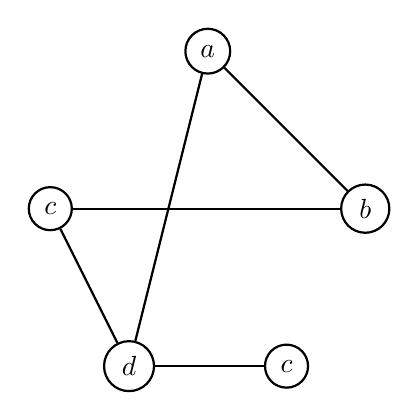
\begin{tikzpicture}
      \begin{scope}[every node/.style={circle,thick,draw}]
        \node (a) at (2,4) {$a$};
        \node (b) at (4,2) {$b$};
        \node (c) at (3,0) {$c$};
        \node (d) at (1,0) {$d$};
        \node (z) at (0,2) {$c$};
      \end{scope}
      \begin{scope}[every edge/.style={draw=black,thick}]
        \path (a) edge (b);
        \path (a) edge (d);
        \path (b) edge (z);
        \path (c) edge (d);
        \path (d) edge (z);
      \end{scope}
    \end{tikzpicture}
  \end{adjustbox}
  \vspace{0.1cm}
  \begin{block}{Exercise}
	Determine the vertex set, edge set and adacency list of this graph.
  \end{block}
  
  \citeurl{global.oup.com/booksites/content/9780198507185/}
\end{frame}


\begin{frame}{Degree of a vertex}

	\begin{definition}
		The degree of a vertex is the number of edges that contain it.
	\end{definition}
	
	  
    \begin{center}
      \begin{columns}
    \begin{column}{0.08\textwidth}
    
    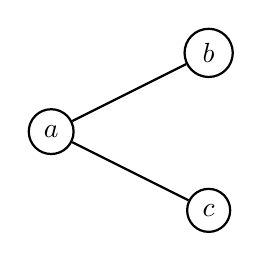
\begin{tikzpicture}
      \begin{scope}[every node/.style={circle,thick,draw}]
        \node (a) at (0,0) {$a$};
        \node (b) at (2,1) {$b$};
        \node (c) at (2,-1) {$c$};
      \end{scope}
      \begin{scope}[every edge/.style={draw=black,thick}]
        \path (a) edge (b);
        \path (a) edge (c);
      \end{scope}
    \end{tikzpicture}
    \end{column}
    \begin{column}{0.5\textwidth}
        The degree of the vertex $a$ is 2.
    \end{column}
    \end{columns}
    \end{center}

	
	
    \begin{block}{Exercise}
	  For each of the vertices on the previous slide, determine its degree.
    \end{block}

\end{frame}


\section{Trees}

\section{Paths and Cycles}

\section{Colouring}

\section{Sorting}

\section{Searching}

\section{Shortest Paths}